\documentclass{article}

\usepackage{graphicx}
\usepackage{tikz}
\usepackage{tikzsymbols}
\usetikzlibrary{calc,patterns,shapes.geometric}
\pagestyle{empty}
\usepackage[margin=0pt]{geometry}
\geometry{papersize={14in,12in}}

\def\centerarc[#1](#2)(#3:#4:#5){\draw[#1] ($(#2)+({#5*cos(#3)},{#5*sin(#3)})$) arc (#3:#4:#5);}

\begin{document}
	\begin{figure}
		\centering
		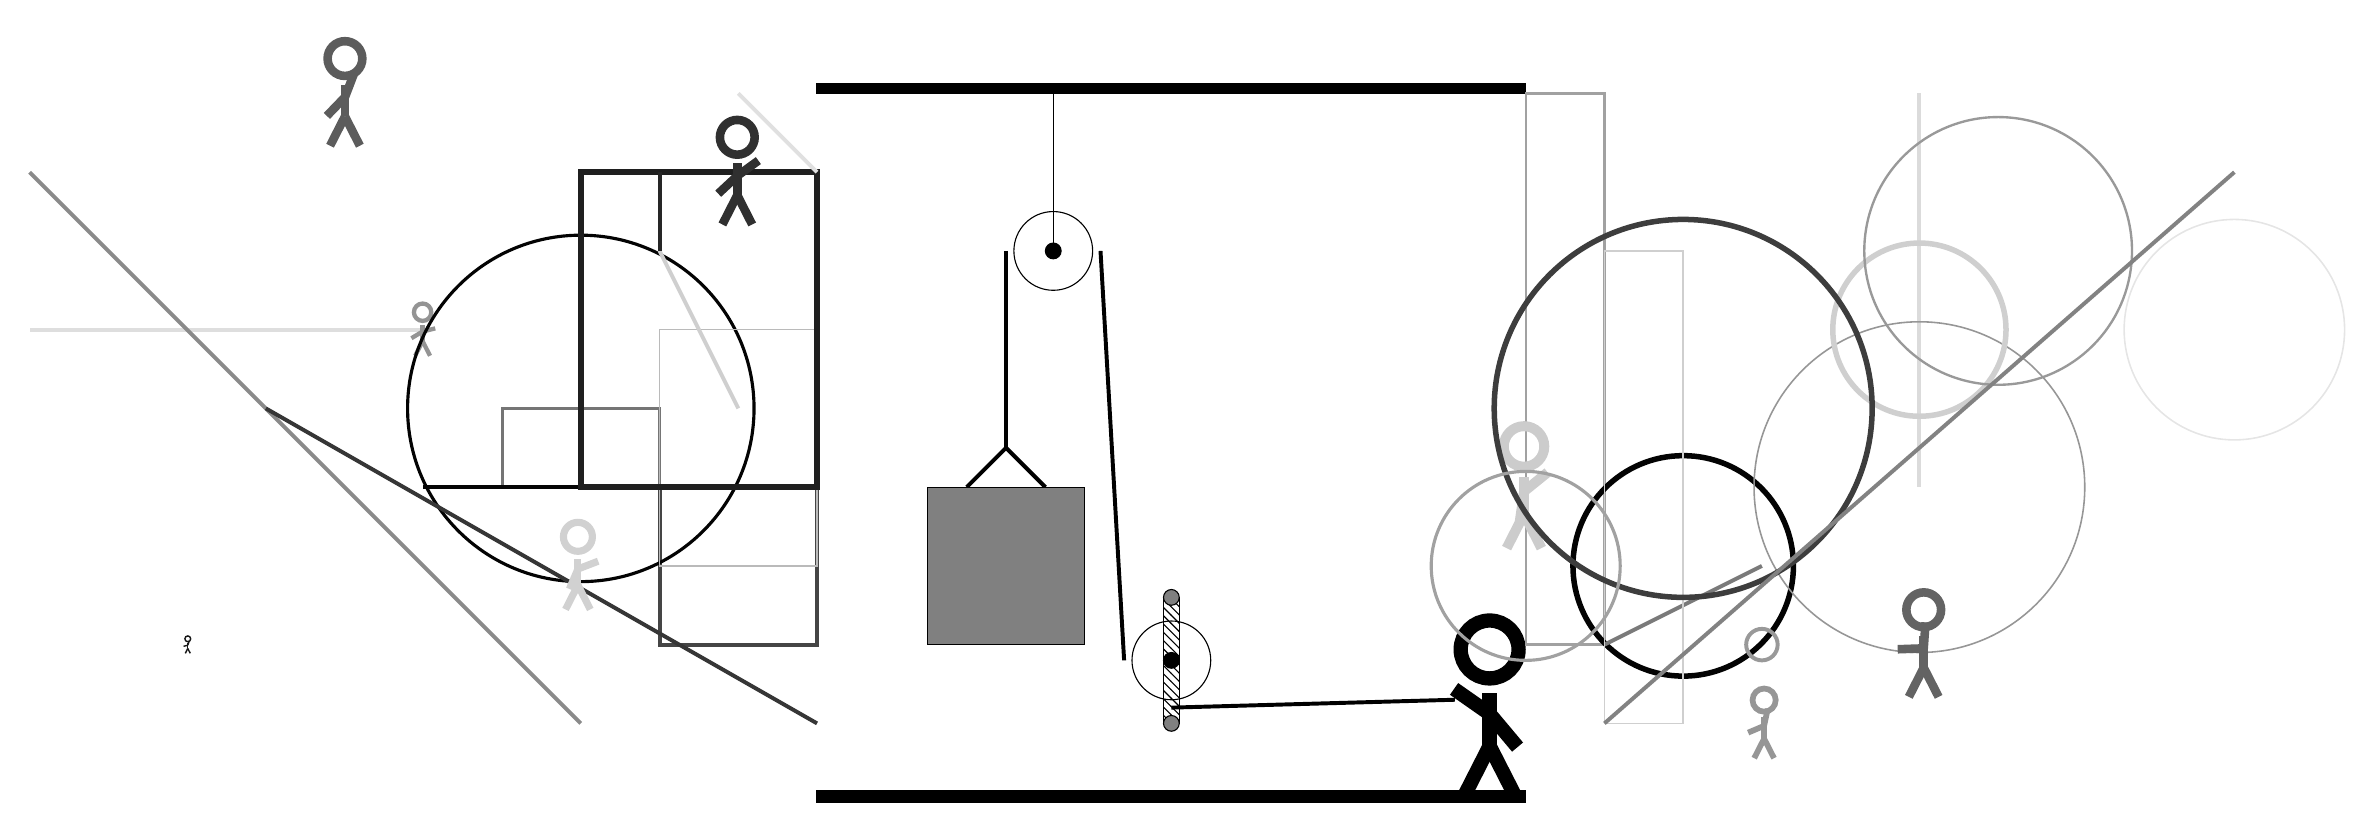
\begin{tikzpicture}
			%%%%% START %%%%%
			
			\draw[fill=black] (-2, 9) rectangle (7, 9.125);
			
			\draw (1, 7) circle (0.5);
			\draw[fill=black] (1, 7) circle (0.1);
			\draw (1, 9) -- (1, 7);
			
			\draw[fill=white](2.5, 1.8) circle (0.5);
			\draw[fill=black] (2.5, 1.8) circle (0.1);
			\draw[pattern=north west lines, pattern color=black] (2.4, 2.6) rectangle (2.6, 1.0);
			\draw[fill=black!50] (2.5, 2.6) circle (0.1);
			\draw[fill=black!50] (2.5, 1.0) circle (0.1);
			
			\draw[line width=0.5mm] (-0.1, 4.0) -- (0.4, 4.5) -- (0.9, 4.0);
			\draw[fill=black!50] (-0.6, 4.0) rectangle (1.4, 2.0);
			
			\draw[line width=0.5mm] (0.4, 7) -- (0.4, 4.5);
			\centerarc[line width=0.5mm](1, 7)(0:180:0.6);
			\draw[line width=0.5mm](1.6, 7) -- (1.9, 1.8);
			\centerarc[line width=0.5mm](2.5, 1.8)(180:270:0.6);
			\draw[line width=0.5mm](2.5, 1.2) -- (6.1, 1.3);
			
			\node at (6.5, 1.2) {\Strichmaxerl[10][-35][-50]};
			
			\node[line width=0.7mm, color=black!41] at (10, 1) {\Strichmaxerl[4][23][78]};
			
			\draw[line width=0.3mm, color=black!37] (8, 2) rectangle (7, 9);
			\draw [line width=0.7mm, color=black!99](9, 3) circle (1.4);
			\draw[line width=0.5mm, color=black!13](-7, 6) -- (-12, 6);
			\draw[line width=0.4mm, color=black!54] (-4, 4) rectangle (-6, 5);
			\draw[line width=0.5mm, color=black!14](12, 9) -- (12, 4);
			
			\draw[line width=0.5mm, color=black!52](8, 2) -- (10, 3);
			\draw [line width=0.2mm, color=black!41](12, 4) circle (2.1);
			\node[line width=0.6mm, color=black!42] at (-7, 6) {\Strichmaxerl[3][31][14]};
			\node[line width=0.7mm, color=black!64] at (-8, 9) {\Strichmaxerl[6][46][69]};
			\draw[line width=0.5mm, color=black!73] (-4, 2) rectangle (-2, 4);
			
			\draw [line width=0.7mm, color=black!19](12, 6) circle (1.1);
			\node[line width=0.2mm, color=black!91] at (-10, 2) {\Strichmaxerl[1][14][71]};
			\draw[line width=0.5mm, color=black!46](-5, 1) -- (-12, 8);
			\draw[line width=0.5mm, color=black!98](-4, 4) -- (-7, 4);
			\draw [line width=0.4mm, color=black!99](-5, 5) circle (2.2);
			
			\draw[line width=0.2mm, color=black!19] (8, 1) rectangle (9, 7);
			\draw[line width=0.2mm, color=black!27] (-2, 6) rectangle (-4, 3);
			\draw[line width=0.5mm, color=black!19](-3, 5) -- (-4, 7);
			\draw[line width=0.7mm, color=black!88] (-2, 8) rectangle (-5, 4);
			\draw [line width=0.3mm, color=black!40](13, 7) circle (1.7);
			
			\node[line width=0.2mm, color=black!81] at (-3, 8) {\Strichmaxerl[6][43][36]};
			\draw [line width=0.2mm, color=black!10](16, 6) circle (1.4);
			\draw[line width=0.5mm, color=black!79](-2, 1) -- (-9, 5);
			\node[line width=0.6mm, color=black!20] at (7, 4) {\Strichmaxerl[7][82][39]};
			\draw [line width=0.7mm, color=black!76](9, 5) circle (2.4);
			
			\draw[line width=0.5mm, color=black!49](8, 1) -- (16, 8);
			\node[line width=0.2mm, color=black!18] at (-5, 3) {\Strichmaxerl[5][67][21]};
			
			\node[line width=0.7mm, color=black!61] at (12, 2) {\Strichmaxerl[6][2][86]};
			\draw[line width=0.5mm, color=black!12](-2, 8) -- (-3, 9);
			\draw [line width=0.4mm, color=black!37](7, 3) circle (1.2);
			\draw [line width=0.5mm, color=black!40](10, 2) circle (0.2);
			\draw[line width=0.5mm, color=black!85](-4, 8) -- (-4, 7);
			
			\draw[fill=black] (-2, 0) rectangle (7, 0.15);
			
			%%%%% END %%%%%
		\end{tikzpicture}
	\end{figure}	
\end{document}